\scanpage{7}
\mspage{2}

comme l'unique élément de \({}_2(X_S)\) qui est fixe par $\operatorname{Aut}(X_S)\simeq\mathbb Z/4\mathbb Z$. En fait
\inserted{\[
(X_S)^{\unsure{i}}\overset{\unsure{\mathrm{def}}}{\unsure{=}}\{x\in X_S\deleted{\}} \mid ix=x\}=\{e,\eta_S\}
\]}
\deleted{\unsure{$X$}} La surface top. $X_S$ a une déc. cell. \inserted{\unsure{can.}} \inserted{\unsure{can. Aut.}} avec 1 sommet $e$, deux arêtes, une face, correspondant aux deux mailles du réseau $\Gamma_S$.

On considère $X_S$ comme muni de cette décomposition. Parfois c'est l'image inv. de celle-ci par $2\operatorname{id}_{X_S}$ qui est plus commode, 4 sommets (formant \({}_2(X_S)\)), \deleted{quatre} \inserted{huit} arêtes, \deleted{(\uline{NB} \unsure{le}} \inserted{4} faces. On peut considérer $\mathbb Z/4\mathbb Z\simeq\mu_4(\mathbb C)$ comme le groupe d'automorphismes commun de ces deux structures cellulaires.

\figure{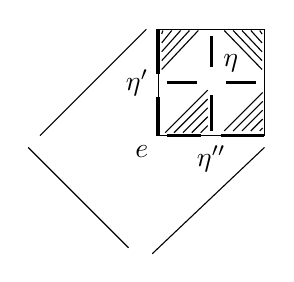
\begin{tikzpicture}[scale=.75]
\draw (-2,0)--(-.2,1.8);
\draw (-2.2,-.2)--(-.5,-1.9);
\draw (-.1,-2)--(1.8,-.2);
\draw (0,0) rectangle (1.8,1.8);
\draw[densely dashed] (0,1.8)--(1.8,1.8)--(1.8,0);
\draw[line width=1.2pt] (0,0)--(0,.65) (0,1.05)--(0,1.8) (.15,0)--(.72,0) (1.06,0)--(1.8,0);
\draw[line width=1.2pt] (.9,.08)--(.9,.69) (.9,1.16)--(.9,1.68) (.15,.9)--(.65,.9) (1.15,.9)--(1.65,.9);
\foreach \t in {.12,.27,.42,.57,.72}{
 \draw[thin] (\t,.05)--(.84,.89-\t);
 \draw[thin] (.06,1+\t)--(.8-\t,1.78);
 \draw[thin] (1+\t,1.78)--(1.76,1+\t);
 \draw[thin] (1+\t,.08)--(1.77,.85-\t);
}
\node[below left] at (0,0) {$e$};
\node[left] at (0,.9) {$\eta'$};
\node[below] at (.9,0) {$\eta''$};
\node[above right] at (.94,.92) {$\unsure{\eta}$};
\end{tikzpicture}}

La deuxième est mieux adaptée pour la description du quotient
\[
\deleted{\unsure{X}\mathbb E\ell(\unsure{S})}\quad X_S/\pm1
\]
qui est une sphère, subdivisée en \deleted{deux} \inserted{faces} \unsure{carrés}, se raccordant suivant un équateur \deleted{carré}, subdivisé en quatre arêtes par $e^{\unsure{\natural}},\eta^{\unsure{\natural}},\eta'^{\unsure{\natural}},\eta''^{\unsure{\natural}}$.

\figure{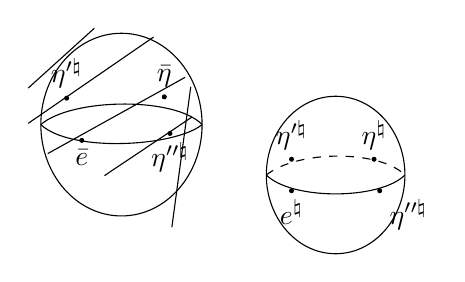
\begin{tikzpicture}[scale=.8]
\begin{scope}
\draw (0,0) ellipse (1.28 and 1.45);
\draw (-1.28,0) .. controls (-.8,.42) and (.85,.45) .. (1.28,0);
\draw (-1.28,0) .. controls (-.8,-.45) and (.85,-.35) .. (1.28,0);
\fill (-.63,-.25) circle (.04) node[below] {$\unsure{\bar e}$};
\fill (-.87,.42) circle (.04) node[above] {$\unsure{\eta'^\natural}$};
\fill (.68,.44) circle (.04) node[above] {$\unsure{\bar\eta}$};
\fill (.77,-.14) circle (.04) node[below] {$\unsure{\eta''^\natural}$};
\draw (-1.48,.58)--(-.43,1.53) (-1.48,.02)--(.51,1.39) (-1.17,-.46)--(1.01,.75) (-.27,-.81)--(1.12,.12) (1.1,.6)--(.8,-1.63);
\end{scope}
\begin{scope}[xshift=3.4cm,yshift=-.8cm]
\draw (0,0) ellipse (1.1 and 1.25);
\draw[dashed] (-1.1,0) .. controls (-.6,.4) and (.7,.4) .. (1.1,0);
\draw (-1.1,0) .. controls (-.7,-.4) and (.7,-.4) .. (1.1,0);
\fill (-.7,.25) circle (.04) node[above] {$\unsure{\eta'^\natural}$};
\fill (.61,.25) circle (.04) node[above] {$\unsure{\eta^\natural}$};
\fill (-.7,-.25) circle (.04) node[below] {$\unsure{e^\natural}$};
\fill (.7,-.25) circle (.04) node[below right] {$\unsure{\eta''^\natural}$};
\end{scope}
\end{tikzpicture}}

\margin{6}
